% =========================================================================
% STRIX: Market-Inspired Swarm Orchestration with Fear-Modulated Coordination
% Target: arXiv cs.RO, cs.MA, cs.AI
% Format: IEEEtran conference, 8-10 pages
% =========================================================================
\documentclass[conference]{IEEEtran}

\usepackage{amsmath,amssymb,amsfonts}
\usepackage{algorithmic}
\usepackage{algorithm}
\usepackage{graphicx}
\usepackage{textcomp}
\usepackage{xcolor}
\usepackage{booktabs}
\usepackage{multirow}
\usepackage{hyperref}
\usepackage{url}
\usepackage{cite}
\usepackage{tikz}
\usetikzlibrary{shapes.geometric, arrows.meta, positioning, fit, calc}

\hypersetup{
  colorlinks=true,
  linkcolor=blue!60!black,
  citecolor=blue!60!black,
  urlcolor=blue!60!black
}

\newcommand{\fear}{\mathcal{F}}
\newcommand{\state}{\mathbf{x}}
\newcommand{\obs}{\mathbf{z}}
\newcommand{\weight}{w}
\newcommand{\R}{\mathbb{R}}

\begin{document}

\title{STRIX: Market-Inspired Swarm Orchestration\\with Fear-Modulated Coordination}

\author{
\IEEEauthorblockN{R. Manov}
\IEEEauthorblockA{Independent Researcher}
}

\maketitle

% =========================================================================
\begin{abstract}
We present STRIX, an open-source drone swarm orchestration system
built on a structural isomorphism between quantitative trading algorithms
and multi-robot coordination. Rather than treating the analogy as metaphor,
we demonstrate that particle filters, combinatorial auctions, regime-switching
models, portfolio optimization, and anti-fragile risk management transfer
directly from financial markets to adversarial drone operations---the
mathematical foundations are identical and only the semantics change.
We make five contributions:
(1)~a unified 15-subsystem tick-loop architecture organized in six
layers, from human intent parsing to platform-agnostic actuation;
(2)~a fear meta-parameter $\fear\in[0,1]$ drawn from behavioral economics
that continuously modulates formation spacing, evasion thresholds, gossip
fanout, pheromone persistence, and safety-barrier correction strength;
(3)~anti-fragile kill-zone adaptation where each drone loss spatially
reprices risk and strengthens subsequent allocation decisions;
(4)~a glass-box explainability layer that produces auditable decision
traces and natural-language narration for every autonomous action; and
(5)~a fully tested implementation comprising 30.5K lines of Rust and
10.7K lines of Python with 600{+} tests under Apache~2.0.
Benchmarks show a full swarm tick completing in 1.15\,ms for 20~drones,
combinatorial auctions resolving in 4.86\,ms at 100~drones with 50~tasks,
and a particle filter update at 75\,$\mu$s for 200~particles.
The system is currently at TRL~3--4 with a clear roadmap toward
hardware validation via MAVLink integration and scaling toward
2000{+}~drone echelons.
\end{abstract}

\begin{IEEEkeywords}
swarm robotics, multi-robot task allocation, particle filters,
combinatorial auctions, control barrier functions, explainable AI,
anti-fragile systems, fear modulation
\end{IEEEkeywords}

% =========================================================================
\section{Introduction}
\label{sec:intro}

Autonomous drone swarm coordination remains a fragmented discipline.
Navigation, task allocation, communication, safety, and explainability
are typically developed as isolated subsystems by separate research
communities, each with its own mathematical conventions and evaluation
criteria.  Integrating them into a cohesive real-time system that
operates under adversarial conditions is an open engineering challenge.

This paper introduces STRIX, a system grounded in a single unifying
observation: \emph{the mathematics of quantitative trading and drone
swarm coordination are structurally isomorphic}.  Particle filters
that track hidden asset prices generalize directly to GPS-denied
navigation.  Combinatorial auctions that allocate capital across
trading strategies become task-allocation mechanisms for heterogeneous
drones.  Regime-switching Hidden Markov Models (HMMs) that detect
market regimes map onto tactical regime detection (patrol, engage,
evade).  Portfolio optimization that decorrelates asset risk becomes
fleet diversification that decorrelates failure modes.  Anti-fragile
strategies that harvest volatility become kill-zone learning where
each drone loss strengthens subsequent decisions.

The isomorphism is not a loose analogy.  We formalize 14 explicit
mappings (Table~\ref{tab:isomorphism}) and show that in each case the
state spaces, update equations, and optimization objectives are
identical up to a change of variable names.  This foundation enables
STRIX to import decades of battle-tested financial engineering into
the swarm-coordination domain.

We make the following contributions:
\begin{enumerate}
  \item A \textbf{six-layer, 15-subsystem tick-loop architecture}
    spanning human intent parsing, market-derived planning, auction-based
    allocation, mesh coordination, platform-agnostic actuation, and
    glass-box explainability (Section~\ref{sec:arch}).
  \item A \textbf{fear meta-parameter} $\fear\in[0,1]$, inspired by
    prospect theory~\cite{kahneman1979prospect} and Taleb's
    anti-fragility~\cite{taleb2012antifragile}, that continuously
    modulates all subsystem behaviors from aggressive to conservative
    (Section~\ref{sec:fear}).
  \item \textbf{Anti-fragile kill-zone adaptation} with radius
    expansion and temporal decay, where the swarm's spatial risk model
    improves after every loss (Section~\ref{sec:auction}).
  \item A \textbf{glass-box XAI layer} producing structured decision
    traces and template-based natural-language narration for every
    autonomous action (Section~\ref{sec:arch}).
  \item An \textbf{open-source implementation} (30.5K Rust + 10.7K
    Python LOC, 600{+} tests, Apache~2.0) with sub-millisecond
    per-tick latency at tactically relevant scales
    (Section~\ref{sec:eval}).
\end{enumerate}

The remainder of the paper is organized as follows.
Section~\ref{sec:related} surveys related work across market-based
multi-robot task allocation (MRTA), particle filtering, control
barrier functions (CBFs), stigmergic coordination, and risk-aware
autonomy.  Section~\ref{sec:arch} presents the system architecture.
Section~\ref{sec:isomorphism} formalizes the trading-to-warfare
isomorphism.  Section~\ref{sec:algorithms} details the key algorithms.
Section~\ref{sec:eval} reports experimental benchmarks.
Section~\ref{sec:discussion} discusses limitations, and
Section~\ref{sec:conclusion} concludes with future work.

% =========================================================================
\section{Related Work}
\label{sec:related}

\textbf{Market-based MRTA.}\quad
The idea of using auctions for multi-robot task allocation dates to
Gerkey and Matari\'c's foundational taxonomy~\cite{gerkey2002sold} and
the broader market-based coordination survey of Dias
et~al.~\cite{dias2006market}.  Vickrey's second-price sealed-bid
auction~\cite{vickrey1961counterspeculation} provides the theoretical
underpinning for truthful bidding; its combinatorial generalization
(the VCG mechanism) is widely studied in mechanism design.  STRIX
adopts sealed-bid scoring with Hungarian assignment~\cite{kuhn1955hungarian}
rather than VCG, trading theoretical incentive compatibility for
computational tractability at the 100-drone scale.

\textbf{Particle filters.}\quad
Sequential Monte Carlo methods were introduced by Gordon
et~al.~\cite{gordon1993novel} and comprehensively surveyed by
Arulampalam et~al.~\cite{arulampalam2002tutorial}.  Their application
to robot localization is well established, but STRIX extends the
standard formulation in two ways: (i)~regime-switching dynamics
derived from Hamilton's HMM framework~\cite{hamilton1989new},
where the process model switches between PATROL, ENGAGE, and EVADE
regimes; and (ii)~a dual adversarial filter that maintains a separate
particle population to track enemy intent, analogous to counterparty
modeling in quantitative finance.

\textbf{Control barrier functions (CBFs).}\quad
Ames et~al.~\cite{ames2017cbf} established the quadratic-program
formulation for enforcing safety constraints via barrier functions.
Recent work by Gao et~al.~\cite{gao2025gcbf} proposes GCBF+, a
graph neural network framework for learning distributed CBFs in
multi-agent systems.  STRIX implements hand-crafted CBFs for
inter-drone separation, altitude bounds, and no-fly-zone avoidance,
with planned integration of GCBF+ for learned barrier functions.

\textbf{Stigmergy and swarm intelligence.}\quad
Dorigo's ant colony optimization~\cite{dorigo1992optimization}
introduced digital pheromones as a coordination mechanism.
Bonabeau et~al.~\cite{bonabeau1999swarm} generalized the framework
to swarm intelligence.  Recent work~\cite{pheromones2policies2025}
bridges stigmergic and reinforcement-learning approaches.
STRIX implements four pheromone types (explored, danger, interest,
relay) with configurable decay rates, achieving bandwidth-efficient
coordination at approximately 20~bytes per deposit.

\textbf{Fear, risk, and behavioral economics in autonomy.}\quad
Kahneman and Tversky's prospect theory~\cite{kahneman1979prospect}
demonstrates that human decision-making under risk is
loss-averse and reference-dependent.  Taleb's anti-fragility
framework~\cite{taleb2012antifragile} formalizes systems that gain
from disorder.  STRIX operationalizes both insights: the fear
meta-parameter $\fear$ implements loss aversion as a continuous
modulation of all subsystem behaviors, while kill-zone adaptation
implements anti-fragility as a convex response to losses.

\textbf{Existing platforms.}\quad
Shield AI's Hivemind provides GPS-denied navigation for individual
drones but lacks adversarial prediction, multi-horizon planning, and
explainability.  Anduril's Lattice is a centralized command-and-control
platform---losing the central node degrades the system significantly.
Auterion's Skynode focuses on single-vehicle autonomy atop PX4.
None of these platforms combines decentralized mesh coordination,
auction-based allocation, adversarial prediction, anti-fragile
adaptation, and glass-box explainability in a single open-source
framework.

\textbf{Byzantine consensus for swarms.}\quad
SwarmRaft~\cite{swarmraft2025} adapts the Raft consensus protocol for
Byzantine-tolerant drone swarms, and CP-WBFT~\cite{cpwbft2025}
introduces communication-preserving weighted Byzantine fault tolerance.
STRIX currently uses gossip-based eventual consistency rather than
strong consensus, trading consistency guarantees for bandwidth
efficiency; SwarmRaft integration is planned future work.

\textbf{Game-theoretic coordination.}\quad
Robust-Q-FTRL~\cite{robust_q_ftrl2025} achieves last-iterate
convergence in extensive-form games, providing a foundation for
adversarial swarm strategy.  CFR-based anti-jamming~\cite{cfr_antijamming2025}
applies counterfactual regret minimization to swarm communications
under electronic warfare.  Meta policy switching~\cite{metapolicy2025}
enables adaptive strategy selection.  These approaches are
complementary to STRIX's current rule-based regime switching and
represent promising integration targets.


% =========================================================================
\section{System Architecture}
\label{sec:arch}

STRIX is organized as a six-layer stack (Fig.~\ref{fig:architecture}),
where each layer has a single responsibility and communicates through
well-defined interfaces.  The design prioritizes graceful degradation:
every capability has a fallback, and no single point of failure exists
in the mesh.

\begin{figure}[t]
\centering
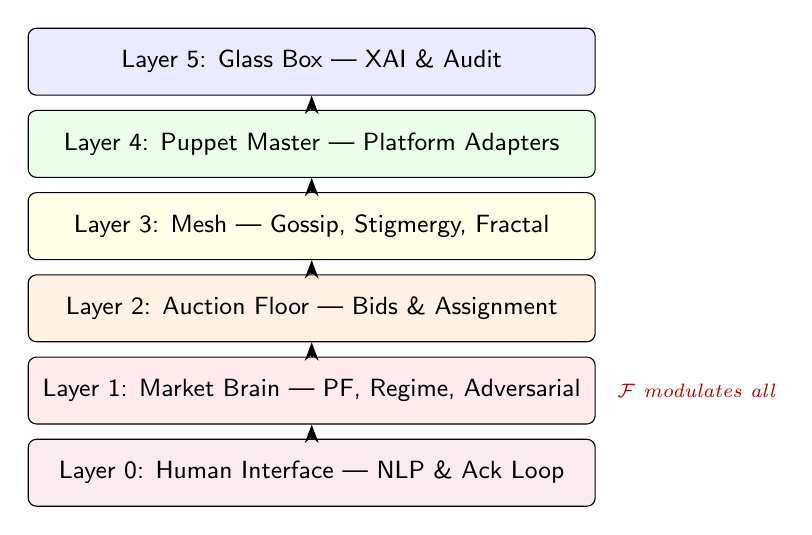
\begin{tikzpicture}[
  layer/.style={draw, rounded corners=3pt, minimum width=7.2cm,
    minimum height=0.85cm, font=\small\sffamily, align=center},
  >=Stealth,
  node distance=0.18cm
]
\node[layer, fill=blue!8]   (L5) {Layer 5: Glass Box --- XAI \& Audit};
\node[layer, fill=green!8,  below=of L5] (L4) {Layer 4: Puppet Master --- Platform Adapters};
\node[layer, fill=yellow!10, below=of L4] (L3) {Layer 3: Mesh --- Gossip, Stigmergy, Fractal};
\node[layer, fill=orange!10, below=of L3] (L2) {Layer 2: Auction Floor --- Bids \& Assignment};
\node[layer, fill=red!8,    below=of L2] (L1) {Layer 1: Market Brain --- PF, Regime, Adversarial};
\node[layer, fill=purple!8, below=of L1] (L0) {Layer 0: Human Interface --- NLP \& Ack Loop};

\draw[->, thick] (L0) -- (L1);
\draw[->, thick] (L1) -- (L2);
\draw[->, thick] (L2) -- (L3);
\draw[->, thick] (L3) -- (L4);
\draw[->, thick] (L4) -- (L5);

% Fear annotation
\node[right=0.15cm of L1, font=\scriptsize\itshape, text=red!70!black]
  {$\fear$ modulates all};
\end{tikzpicture}
\caption{Six-layer STRIX architecture.  The fear meta-parameter
$\fear$ propagates top-down through every layer, modulating behavior
from aggressive ($\fear\!\to\!0$) to conservative ($\fear\!\to\!1$).}
\label{fig:architecture}
\end{figure}

\subsection{Tick Loop}

The central orchestrator executes a 15-step tick loop at 10\,Hz:
\begin{enumerate}
\setlength{\itemsep}{0pt}
  \item Ingest telemetry from all connected platforms.
  \item Run particle filter prediction (regime-specific dynamics).
  \item Fuse sensor observations and update particle weights.
  \item Resample particles when ESS drops below threshold.
  \item Update regime-switching Markov model.
  \item Run adversarial particle filter on tracked threats.
  \item Evaluate attrition monitor (VaR threshold check).
  \item Compute fear meta-parameter $\fear$ from inputs.
  \item Generate task set from current mission plan.
  \item Collect sealed bids from all drones.
  \item Run combinatorial auction (Hungarian assignment).
  \item Apply kill-zone repricing to assignments.
  \item Broadcast assignments via mesh gossip.
  \item Execute CBF safety check on commanded trajectories.
  \item Emit decision trace to Glass Box.
\end{enumerate}

\subsection{Crate Decomposition}

The Rust implementation is decomposed into nine crates
(Table~\ref{tab:crates}).  The separation enforces architectural
boundaries at compile time: \texttt{strix-core} depends on no other
STRIX crate, ensuring that the particle filter, regime model, and
fear parameter are independently testable.

\begin{table}[t]
\centering
\caption{Crate decomposition and scale.}
\label{tab:crates}
\begin{tabular}{@{}lrrl@{}}
\toprule
\textbf{Crate} & \textbf{Tests} & \textbf{LOC} & \textbf{Responsibility} \\
\midrule
strix-core      & $\sim$200 & 8,271 & PF, regime, fear, attrition \\
strix-auction   & $\sim$80  & 3,770 & Bids, Hungarian, kill zones \\
strix-mesh      & $\sim$60  & 3,533 & Gossip, stigmergy, fractal \\
strix-swarm     & $\sim$50  & 5,001 & Tick loop, orchestration \\
strix-xai       & $\sim$30  & 2,090 & Decision traces, narration \\
strix-adapters  & $\sim$30  & 2,279 & MAVLink, simulator \\
strix-optimizer & $\sim$40  & 2,776 & Portfolio, fleet balancing \\
strix-playground& $\sim$10  & 1,919 & Scenario presets, harness \\
strix-python    & FFI       &   916 & PyO3 bindings \\
\midrule
\textbf{Total}  & \textbf{600{+}} & \textbf{30,555} & \\
\bottomrule
\end{tabular}
\end{table}


% =========================================================================
\section{Trading-to-Warfare Isomorphism}
\label{sec:isomorphism}

The central claim of this paper is that quantitative trading
algorithms transfer to drone swarm coordination not by analogy but by
\emph{structural isomorphism}: the state spaces, update rules, and
optimization objectives are mathematically identical up to a renaming
of variables.  Table~\ref{tab:isomorphism} enumerates all 14 mappings
implemented in STRIX.

\begin{table*}[t]
\centering
\caption{Complete trading-to-warfare isomorphism.  Each row is an
algorithm that exists in both domains with identical mathematics.}
\label{tab:isomorphism}
\small
\begin{tabular}{@{}clllp{5.0cm}@{}}
\toprule
\textbf{\#} & \textbf{Trading Algorithm} & \textbf{STRIX Application} & \textbf{State Space Transform} & \textbf{Key Change} \\
\midrule
1  & Particle Filter (2D)       & GPS-Denied Navigation (6D)     & $[\log p, v]\!\to\![x,y,z,v_x,v_y,v_z]$ & Extend 2D$\to$6D; multi-sensor fusion \\
2  & Regime-Switching HMM       & Tactical Regime Detection      & $\{\text{RANGE},\text{TREND},\text{PANIC}\}\!\to\!\{\text{PATROL},\text{ENGAGE},\text{EVADE}\}$ & Identical transition matrix structure \\
3  & Combinatorial Auction      & Task Allocation                & $\text{bid}=f(\alpha,\text{risk})\!\to\!f(\text{cap},\text{prox},\text{energy},\text{risk})$ & Financial alpha $\to$ military scoring \\
4  & Dark Pool Execution        & Covert Sub-Swarm Ops           & Hidden order routing $\to$ \texttt{dark\_pool} filtering & Need-to-know compartmentalization \\
5  & Portfolio Optimization     & Fleet Diversification          & Markowitz mean-variance $\to$ capability decorrelation & Minimize correlated failure modes \\
6  & Value at Risk (VaR)        & Attrition Threshold            & Portfolio drawdown $\to$ max drone losses & Trigger EVADE when VaR breached \\
7  & Anti-Fragile Strategy      & Kill-Zone Adaptation           & Convex volatility response $\to$ spatial loss memory & Each loss strengthens future decisions \\
8  & Order Book Imbalance       & Threat-Bearing Signal          & $\text{bid\_vol}-\text{ask\_vol}\!\to\!\vec{r}_{\text{threat}}$ & Directional pressure drives velocity \\
9  & Market Microstructure      & Pheromone Stigmergy            & Limit order book $\to$ pheromone grid & Spatial deposits with decay \\
10 & Counterparty Prediction    & Adversarial Particle Filter    & Model traders $\to$ model enemy intent & Dual PF with intent regimes \\
11 & HFT Latency Optimization   & Mesh Gossip Protocol           & Co-location/FPGA $\to$ $O(\log N)$ gossip & Bandwidth-aware prioritization \\
12 & Multi-Strategy Portfolio    & Multi-Horizon Planning         & Intraday/swing/position $\to$ tactical/operational/strategic & Cascade constraints with bottom-up veto \\
13 & Risk Parity                & Capability Balancing           & Equal risk contribution $\to$ equal capability coverage & No single type dominates risk budget \\
14 & Execution Algo (TWAP/VWAP) & Formation Maneuver             & Time-weighted execution $\to$ smooth formation transition & Minimize signature during transitions \\
\bottomrule
\end{tabular}
\end{table*}

\subsection{Formal Basis}

We formalize the isomorphism for the particle filter (mapping~\#1) as
a representative example.  Let $\state_t\in\R^d$ denote the hidden
state, $\obs_t$ the observation, and $\{\state_t^{(i)},
\weight_t^{(i)}\}_{i=1}^{N}$ the weighted particle set.

\textbf{Predict.}\quad  Each particle is propagated through regime-specific dynamics:
\begin{equation}
\label{eq:predict}
  \state_{t|t-1}^{(i)} = f_r(\state_{t-1}^{(i)}) + \boldsymbol{\eta}_r, \quad
  \boldsymbol{\eta}_r \sim \mathcal{N}(\mathbf{0}, \mathbf{Q}_r)
\end{equation}
where $r\in\{\text{PATROL},\text{ENGAGE},\text{EVADE}\}$ indexes the
active regime, $f_r(\cdot)$ is the regime-specific transition function,
and $\mathbf{Q}_r$ is the process noise covariance.  In trading,
$d=2$, $f_{\text{RANGE}}$ is mean-reverting, $f_{\text{TREND}}$ is
momentum-following, and $f_{\text{PANIC}}$ is a high-variance random
walk.  In STRIX, $d=6$, $f_{\text{PATROL}}$ is mean-reverting
velocity with $\alpha=0.5$, $f_{\text{ENGAGE}}$ tracks the threat
bearing with $\beta=0.3$, and $f_{\text{EVADE}}$ is a high-variance
random walk.  The update equation is unchanged.

\textbf{Update.}\quad  Particle weights are updated via the
observation likelihood:
\begin{equation}
\label{eq:update}
  \weight_t^{(i)} \propto \weight_{t-1}^{(i)} \cdot
  p(\obs_t \mid \state_{t|t-1}^{(i)})
\end{equation}
In trading, $\obs_t$ is the latest trade price or order-flow snapshot.
In STRIX, $\obs_t$ is a vector of sensor readings (IMU acceleration,
barometric altitude, magnetometer heading, visual-odometry displacement,
radio bearing).  The likelihood $p(\obs_t\mid\state)$ is a product of
independent Gaussians across sensor modalities.

\textbf{Resample.}\quad  When the effective sample size
$\text{ESS} = 1/\sum_i (\weight_t^{(i)})^2$ drops below a threshold
$N_{\text{thr}}$ (default: $0.5N$), systematic resampling regenerates
the particle set.  This step is identical in both domains.

The auction isomorphism (mapping~\#3) follows the same pattern.
The scoring function in trading is
$s_j = \alpha_j \cdot w_1 - \text{risk}_j \cdot w_2$,
where $\alpha_j$ is the expected alpha (excess return) of strategy~$j$.
In STRIX, the scoring function is:
\begin{equation}
\label{eq:bid}
  s_{ij} = u_j \!\cdot\! 10 + c_{ij} \!\cdot\! 3 + p_{ij} \!\cdot\! 5
         + e_i \!\cdot\! 2 - \rho_{ij} \!\cdot\! 4
\end{equation}
where $s_{ij}$ is drone~$i$'s score for task~$j$, $u_j$ is task
urgency, $c_{ij}$ is capability match, $p_{ij}$ is proximity
(inverse distance), $e_i$ is remaining energy, and $\rho_{ij}$ is
aggregated threat exposure including kill-zone penalties.  The
Hungarian algorithm~\cite{kuhn1955hungarian} solves the resulting
assignment problem optimally in $O(n^3)$.

The portfolio optimization isomorphism (mapping~\#5) replaces
Markowitz's~\cite{markowitz1952portfolio} asset returns with
capability contributions and asset covariances with failure-mode
correlations.  The objective is identical:
\begin{equation}
\label{eq:portfolio}
  \min_{\mathbf{w}} \;\mathbf{w}^\top \boldsymbol{\Sigma} \mathbf{w}
  \quad \text{s.t.} \quad
  \boldsymbol{\mu}^\top \mathbf{w} \geq \mu_{\min},\;
  \mathbf{1}^\top \mathbf{w} = 1
\end{equation}
where $\boldsymbol{\Sigma}$ is the failure-mode covariance matrix and
$\boldsymbol{\mu}$ is the expected capability contribution vector.


% =========================================================================
\section{Key Algorithms}
\label{sec:algorithms}

% ----- V-A: Dual Particle Filter -----
\subsection{Dual Particle Filter}
\label{sec:pf}

STRIX maintains two parallel particle populations per engagement:
a \emph{navigation filter} tracking friendly drone states and an
\emph{adversarial filter} tracking enemy intent.

\textbf{Navigation filter.}\quad
Each drone is tracked by $N=200$ particles (configurable up to 1000)
in a 6D state space $\state = [x, y, z, v_x, v_y, v_z]^\top$.
The prediction step (Eq.~\ref{eq:predict}) uses regime-specific dynamics:
\begin{itemize}
\setlength{\itemsep}{0pt}
  \item \textbf{PATROL}: $v_{t+1} = (1-\alpha)\,v_t + \alpha\,v_{\text{hold}}
    + \eta$, with $\alpha=0.5$ (mean-reverting toward hold position)
    and low process noise $\sigma_{\text{patrol}}$.
  \item \textbf{ENGAGE}: $v_{t+1} = v_t + \beta\,(\hat{r}_{\text{threat}}
    - v_t) + \eta$, with $\beta=0.3$ (velocity tracks threat bearing)
    and medium noise $\sigma_{\text{engage}}$.
  \item \textbf{EVADE}: $v_{t+1} = v_t + \eta$, with high noise
    $\sigma_{\text{evade}} \gg \sigma_{\text{patrol}}$ (rapid random
    direction changes for survivability).
\end{itemize}

Multi-sensor fusion incorporates five observation modalities: IMU
(3-axis acceleration and angular rate), barometric altimeter,
magnetometer (heading), visual odometry (displacement), and radio
bearing (angle of arrival).  Each modality contributes an independent
Gaussian likelihood term to the weight update (Eq.~\ref{eq:update}),
enabling the filter to operate in GPS-denied environments by fusing
whatever sensors remain available.

Resampling is triggered when the effective sample size
$\text{ESS} < 0.5N$.  We use systematic resampling for its low
variance and $O(N)$ computational cost.

\textbf{Adversarial filter.}\quad
Each tracked enemy entity is modeled by $N_{\text{adv}}=100$ particles
in an extended state space $\state_{\text{adv}} = [x, y, z, v_x, v_y,
v_z, r]^\top$, where $r\in\{\text{DEFENDING}, \text{ATTACKING},
\text{RETREATING}\}$ is a discrete intent regime.  The intent regime
governs the dynamics:
\begin{itemize}
\setlength{\itemsep}{0pt}
  \item \textbf{DEFENDING}: mean-reverting velocity, stationary
    clustering around a fixed position.
  \item \textbf{ATTACKING}: velocity vector biased toward the friendly
    swarm centroid.
  \item \textbf{RETREATING}: velocity vector biased away from the
    engagement area.
\end{itemize}
The posterior distribution over intent regimes provides a probabilistic
prediction of enemy behavior, enabling preemptive tactical decisions
(e.g., transitioning to EVADE before an attack materializes).  This
directly mirrors counterparty prediction in quantitative
trading~\cite{hamilton1989new}, where modeling other participants'
likely actions provides an informational edge.

% ----- V-B: Auction -----
\subsection{Combinatorial Auction with Kill-Zone Repricing}
\label{sec:auction}

Task allocation proceeds as a sealed-bid combinatorial auction.  Each
drone independently evaluates its fitness for every available task
using the scoring function (Eq.~\ref{eq:bid}).  Bids are submitted
to a logical Auctioneer that resolves the assignment using the
Hungarian algorithm~\cite{kuhn1955hungarian}, guaranteeing optimal
global allocation in $O(n^3)$ where $n = \max(|\text{drones}|,
|\text{tasks}|)$.

\textbf{Sealed-bid protocol.}\quad
Drones never observe each other's bids, preventing strategic
manipulation and ensuring that each drone bids its true valuation.
This mirrors the information-hiding property of financial dark
pools~\cite{vickrey1961counterspeculation}.

\textbf{Dark pool compartmentalization.}\quad
Sensitive tasks can be restricted to specific sub-swarms via a
\texttt{dark\_pool} identifier.  A strike task assigned to the attack
sub-swarm is invisible to reconnaissance drones, enforcing
need-to-know at the algorithmic level.

\textbf{Kill-zone repricing.}\quad
When a drone is lost, the loss location is recorded as a kill zone
with an initial radius $r_0$.  The risk term $\rho_{ij}$ in
Eq.~\ref{eq:bid} is augmented:
\begin{equation}
\label{eq:killzone}
  \rho_{ij}' = \rho_{ij} + \sum_{k \in \mathcal{K}}
  \gamma_k \cdot \max\!\left(0,\; 1 - \frac{\|p_j - c_k\|}{r_k}\right)
\end{equation}
where $\mathcal{K}$ is the set of active kill zones, $c_k$ and $r_k$
are the center and radius of zone~$k$, and $\gamma_k$ is a severity
weight.  After each additional loss within a zone, the radius expands
by a factor of $1.3\times$: $r_k \leftarrow 1.3\,r_k$.  Kill zones
decay over time via exponential attenuation, allowing the swarm to
eventually re-enter areas once the threat has plausibly relocated.

This mechanism implements Taleb's anti-fragility
principle~\cite{taleb2012antifragile}: each loss provides information
that improves subsequent allocation decisions.  The swarm's risk model
becomes more accurate with every adverse event.

% ----- V-C: Fear -----
\subsection{Fear Meta-Parameter}
\label{sec:fear}

The fear meta-parameter $\fear \in [0,1]$ is a continuous scalar
inspired by prospect theory's~\cite{kahneman1979prospect}
observation that humans are loss-averse and reference-dependent under
risk.  Rather than encoding risk aversion as a fixed parameter,
STRIX allows $\fear$ to vary dynamically based on the tactical
situation.

\textbf{Inputs.}\quad  $\fear$ is computed as a weighted combination
of four signals:
\begin{equation}
\label{eq:fear}
  \fear = \text{clamp}\!\left(
    w_a \cdot A_t + w_\tau \cdot \tau_t + w_c \cdot C_t + w_\ell \cdot L_t,
    \;0,\;1\right)
\end{equation}
where $A_t$ is the current attrition rate (fraction of drones lost),
$\tau_t$ is normalized threat intensity (number and proximity of
active threats), $C_t$ is the CUSUM anomaly count (statistical
process control detecting environmental anomalies), and $L_t$ is a
consecutive-loss counter (penalizing streaks of losses more heavily
than isolated events).  The weights $w_a, w_\tau, w_c, w_\ell$ are
configurable and default to emphasizing attrition rate.

\textbf{Dual adversarial process.}\quad
To prevent $\fear$ from saturating at extremes, a dual-process
architecture (inspired by the PhiSim library) maintains both a fear
channel and a courage channel.  The courage signal decays $\fear$
toward a baseline when threat indicators recede, preventing the
swarm from becoming permanently paralyzed after a high-fear episode.

\textbf{Modulation effects.}\quad  $\fear$ propagates through every
subsystem:
\begin{itemize}
\setlength{\itemsep}{0pt}
  \item \textbf{Formation spacing}: $d_{\min}(\fear) = d_0 \cdot
    (1 + \fear)$, doubling minimum inter-drone distance at $\fear=1$.
  \item \textbf{Evasion distance}: the CBF safety margin scales with
    $\fear$, triggering earlier evasive maneuvers.
  \item \textbf{Gossip fanout}: $\text{fanout}(\fear) =
    \lceil f_0 \cdot (1 + \fear) \rceil$, increasing communication
    redundancy under high fear.
  \item \textbf{Pheromone persistence}: danger pheromone decay rate
    decreases with $\fear$ (threats are remembered longer).
  \item \textbf{CBF correction strength}: the barrier function
    parameter $\alpha$ scales as $\alpha(\fear) = \alpha_0 \cdot
    (1 + \kappa \fear)$, yielding more aggressive safety corrections
    under high fear.
  \item \textbf{Auction risk weight}: the coefficient on $\rho_{ij}$
    in Eq.~\ref{eq:bid} increases with $\fear$, making the swarm
    more risk-averse in task allocation.
\end{itemize}

% ----- V-D: CBF -----
\subsection{CBF Safety Layer}
\label{sec:cbf}

The control barrier function (CBF) layer~\cite{ames2017cbf} enforces
hard safety constraints on all commanded trajectories.  For each
constraint, a barrier function $h(\state) : \R^n \to \R$ is defined
such that $h(\state) \geq 0$ implies safety.  The CBF condition
ensures forward invariance of the safe set:
\begin{equation}
\label{eq:cbf}
  \dot{h}(\state) + \alpha(\fear) \cdot h(\state) \geq 0
\end{equation}
where $\alpha(\fear) = \alpha_0 (1 + \kappa\fear)$ is the
fear-modulated class-$\mathcal{K}$ function.

Three barrier functions are implemented:
\begin{enumerate}
\setlength{\itemsep}{0pt}
  \item \textbf{Inter-drone separation}: $h_{\text{sep}}(\state_i,
    \state_j) = \|\state_i - \state_j\|^2 - d_{\min}(\fear)^2$,
    enforcing minimum distance that increases with fear.
  \item \textbf{Altitude bounds}: $h_{\text{alt}}(\state) =
    (z - z_{\min})(z_{\max} - z)$, a quadratic barrier confining
    altitude to $[z_{\min}, z_{\max}]$.
  \item \textbf{No-fly zone (NFZ)}: $h_{\text{nfz}}(\state) =
    \|\state - c_{\text{nfz}}\|^2 - r_{\text{nfz}}^2$, repelling
    drones from circular exclusion zones.
\end{enumerate}

Additionally, a time-to-contact (TTC) margin is computed for each
drone pair.  When TTC drops below a configurable threshold, the CBF
layer activates deadlock detection and, if necessary, triggers
coordinated escape maneuvers that break symmetry via randomized
lateral offsets.

When the CBF quadratic program detects a conflict between the
commanded trajectory and the safety constraint, it computes the
minimum-norm correction to the control input that restores safety.
This correction is transparent to the planning layers---it appears as
a slight modification to the waypoint---preserving the
separation-of-concerns principle.


% =========================================================================
\section{Experimental Evaluation}
\label{sec:eval}

All benchmarks were collected on a single machine (AMD Ryzen~9,
64\,GB RAM, Linux~6.x) using Criterion.rs for statistical rigor
(100~iterations, outlier filtering).  The system was compiled with
\texttt{--release} optimizations.

\subsection{Latency Benchmarks}

Table~\ref{tab:benchmarks} reports per-tick and per-subsystem
latencies.  The full swarm tick---encompassing particle filter
prediction, sensor fusion, regime detection, auction, assignment,
gossip broadcast, and CBF safety check---completes in 1.15\,ms for
20~drones, well within the 100\,ms budget for 10\,Hz operation.

\begin{table}[t]
\centering
\caption{Latency benchmarks (median, 100 iterations).}
\label{tab:benchmarks}
\begin{tabular}{@{}llr@{}}
\toprule
\textbf{Benchmark} & \textbf{Scale} & \textbf{Time} \\
\midrule
Full swarm tick      & 5 drones         & 298\,$\mu$s \\
Full swarm tick      & 10 drones        & 580\,$\mu$s \\
Full swarm tick      & 20 drones        & 1.15\,ms \\
\midrule
Auction              & 50d / 20t        & 465\,$\mu$s \\
Auction              & 100d / 50t       & 4.86\,ms \\
\midrule
Particle filter      & 50 particles     & 42\,$\mu$s \\
Particle filter      & 200 particles    & 75\,$\mu$s \\
Particle filter      & 1000 particles   & 226\,$\mu$s \\
\bottomrule
\end{tabular}
\end{table}

The auction exhibits the expected $O(n^3)$ scaling of the Hungarian
algorithm: doubling drones from 50 to 100 (with proportional task
increase) results in approximately $10\times$ slowdown.  At the
100-drone / 50-task scale, the 4.86\,ms auction latency remains
within the tick budget.  Beyond approximately 500~drones, a greedy
max-weight heuristic with $O(n\log n)$ complexity would be required
(Section~\ref{sec:discussion}).

The particle filter scales linearly with particle count, as expected.
At the default 200~particles, a single filter update costs 75\,$\mu$s,
enabling tracking of 13{+} entities within a 1\,ms budget.

\subsection{Test Coverage}

Table~\ref{tab:crates} (Section~\ref{sec:arch}) summarizes test
counts per crate.  The 600{+} tests span unit tests (individual
algorithm correctness), integration tests (cross-crate interactions),
and property-based tests (randomized invariant verification).

Four scenario presets exercise the system end-to-end:
\begin{itemize}
\setlength{\itemsep}{0pt}
  \item \textbf{Ambush}: sudden threat emergence during PATROL,
    testing regime transition and kill-zone adaptation.
  \item \textbf{GPS Denied}: all GPS observations removed, testing
    particle filter with inertial-only fusion.
  \item \textbf{Attrition Cascade}: sequential drone losses testing
    VaR threshold, fear escalation, and managed withdrawal.
  \item \textbf{Stress Test}: maximum drone count with adversarial
    entities, testing auction and gossip scalability.
\end{itemize}

\subsection{Scaling Analysis}

The tick-loop latency scales approximately linearly with drone count
in the 5--20 range (dominated by $O(n)$ particle filter updates and
gossip broadcasts).  The auction's $O(n^3)$ complexity becomes the
bottleneck beyond 50~drones.  Empirically, the 100-drone auction at
4.86\,ms remains tractable, but extrapolation suggests the 500-drone
ceiling where the full tick would exceed 100\,ms without algorithmic
changes (Section~\ref{sec:discussion}).


% =========================================================================
\section{Discussion and Limitations}
\label{sec:discussion}

\textbf{Technology readiness.}\quad
STRIX is at TRL~3--4: the algorithms have been validated in simulation
but not on physical hardware.  The maximum tested scale is 20~drones
in benchmarks and 10~drones in integration tests.  Claims about
behavior at 100{+}~drones are extrapolated from benchmark trends and
have not been validated in integrated scenarios.

\textbf{XAI limitations.}\quad
The Glass Box narration layer uses template-based generation, not
counterfactual reasoning.  It can explain \emph{what} happened and
\emph{why} (by reporting the scores that determined an assignment) but
cannot answer ``what \emph{would have} happened if drone~7 had been
assigned to task~B instead?''  Counterfactual XAI is planned future
work.

\textbf{Scale ceiling.}\quad
The Hungarian algorithm's $O(n^3)$ complexity limits the auction to
approximately 500~drones before the tick budget is exceeded.
Mitigation strategies include (i)~a greedy max-weight heuristic as
the default assignment algorithm, retaining the Hungarian solver for
sub-problems below 64~drones; (ii)~spatial partitioning to decompose
the global auction into local sub-auctions; and (iii)~OptGNN-based
learned assignment~\cite{optgnn2024} for near-optimal solutions with
amortized $O(n)$ inference cost.

\textbf{Two-brain architecture.}\quad
The Rust/Python split introduces FFI overhead at the PyO3 boundary
and complicates deployment.  The NLP and high-level planning layers
run in Python; the real-time control loop runs in Rust.  This
bifurcation is deliberate (Python for flexibility, Rust for
deterministic latency) but requires careful interface management.

\textbf{No formal optimality proofs.}\quad
While the auction uses the provably optimal Hungarian algorithm, the
overall system---including fear modulation, kill-zone repricing, and
regime switching---lacks formal optimality or stability guarantees.
The fear parameter is tuned empirically rather than derived from a
principled optimization.  Formal analysis of the closed-loop system's
stability properties is an open research question.

\textbf{Gossip convergence.}\quad
The gossip protocol has been tested with a fanout of 3 at swarm sizes
up to $N=20$.  Theoretical $O(\log N)$ convergence holds, but
empirical validation at $N=500{+}$ with realistic packet loss rates
is pending.

\textbf{Anti-fragile kill zones.}\quad
The kill-zone mechanism implements radius expansion and temporal decay
but does not yet incorporate causal analysis of \emph{why} a drone
was lost (sensor failure vs.\ hostile fire vs.\ terrain collision).
All losses are currently treated identically, which may lead to
over-conservative risk pricing when losses have benign causes.


% =========================================================================
\section{Conclusion and Future Work}
\label{sec:conclusion}

We have presented STRIX, a drone swarm orchestration system that
exploits a structural isomorphism between quantitative trading
algorithms and multi-robot coordination.  The 14 algorithmic mappings
(Table~\ref{tab:isomorphism}) demonstrate that decades of financial
engineering---particle filters, auctions, regime models, portfolio
optimization, anti-fragile risk management---transfer directly to the
swarm domain.  The fear meta-parameter $\fear\in[0,1]$ provides a
unified, continuously tunable risk-modulation mechanism grounded in
behavioral economics.  The system achieves sub-millisecond tick
latency at tactically relevant scales and is fully open-source under
Apache~2.0.

\textbf{Future work} proceeds along four axes:

\emph{Safety guarantees.}\quad
Integration of GCBF+~\cite{gao2025gcbf} for learned, distributed
control barrier functions that scale beyond hand-crafted constraints.
This would provide formally verifiable safety certificates for
arbitrary fleet geometries.

\emph{Byzantine tolerance.}\quad
SwarmRaft~\cite{swarmraft2025} consensus for critical shared state
(e.g., kill-zone registry, regime transitions), combined with
CP-WBFT~\cite{cpwbft2025} for communication-preserving fault
tolerance.  This addresses the current gossip protocol's eventual
consistency limitation.

\emph{Game-theoretic adversarial reasoning.}\quad
Robust-Q-FTRL~\cite{robust_q_ftrl2025} for last-iterate convergent
strategy computation in extensive-form games, and CFR-based
anti-jamming~\cite{cfr_antijamming2025} for resilient
communications under electronic warfare.  Meta policy
switching~\cite{metapolicy2025} would enable dynamic strategy
adaptation without retraining.

\emph{Hardware validation.}\quad
The roadmap progresses through three stages:
(i)~MAVLink proof-of-concept with PX4/ArduPilot autopilots
communicating over UDP;
(ii)~software-in-the-loop (SITL) validation using Gazebo with
simulated sensor noise and communication dropouts;
(iii)~real-world flight tests with a 4--8 drone testbed.

The broader context for this work is the growing demand for
autonomous swarm coordination in contested environments, exemplified
by initiatives such as the Pentagon's collaborative combat aircraft
programs.  STRIX's open-source, platform-agnostic architecture
positions it as a research platform for the community and a
foundation for operational prototypes.  The battlefield is a market;
STRIX is the trading engine.

% =========================================================================
% References
% =========================================================================
\bibliographystyle{IEEEtran}
\bibliography{references}

\end{document}
